\chapter{\uppercase{First Publishable Paper} \label{chapter:02}}

\section{Summary}
This is where the abstract of a publication would go.

\section{First Section of Publication}
Repeat yourself.  Yep, that's fun.  Hope you planned well.  An example of
planning with equations.

\begin{equation}
\label{eq:chap2_example_eq}
  \omega_{jk}\left(x\right) =
  \begin{cases}
  \hfil 0                                        & \hfil x \leq \xi_{j} \\
  \frac{x - \xi_{j}} {\xi_{j + k - 1} - \xi_{j}} & \xi_{j} < x < \xi_{j+ k - 1} \\
  \hfil 1                                        & \hfil \xi_{j + k - 1} \leq x
  \end{cases}.
\end{equation}

This equation, equation \eqref{eq:chap2_example_eq}, is referenced via the \LaTeX\
label {\tt eq:chap2\_example\_eq}.  Now, if this equation is part of what will be
Chapter~\ref{chapter:03}, then make sure you have a qualifier in the equation
label, such as {\tt eq:chap2\_example\_eq} and {\tt eq:chap3\_example\_eq}, to
keep the references accurate.


\section{Floats}

So, tables and figures\ldots
\lipsum

\subsection{Tables}

\lipsum[1]

\ctable[caption = {long caption goes here with lots of detail},
cap = {Short caption for List of Tables here},
label = {tab:recovered_surfaces}]{lccc}{}{ \FL
  Error & col1 & col2 & col3 \ML
  0    & 96.25 & 95.00 & 98.70 \NN
  0.01 & 93.75 & 48.75 & 52.00 \NN
  0.02 & 93.75 & 39.75 & 42.40 \NN  
  0.05 & 91.75 & 28.00 & 30.52 \NN  
  0.10 & 91.00 & 17.50 & 19.23 \NN 
  0.25 & 84.75 & 10.25 & 12.09 \NN  
  0.50 & 63.50 & 05.50 & 08.66 \LL
}

\lipsum

\begin{figure}
\centering
  \begin{subfigure}[t]{0.48\linewidth}
  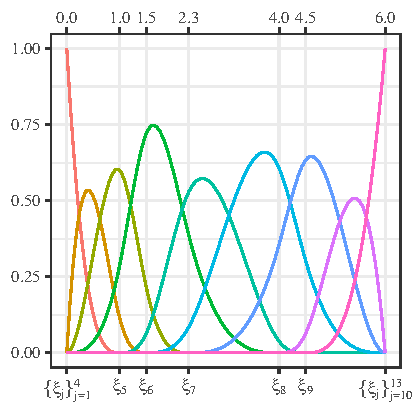
\includegraphics[width=\linewidth]{figures/a}
  \caption{\label{fig:graphic_a}}
  \end{subfigure}
  ~
  \begin{subfigure}[t]{0.48\linewidth}
  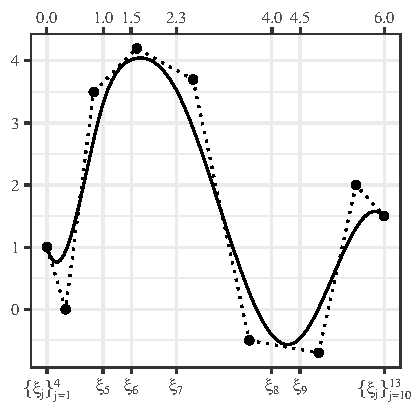
\includegraphics[width=\linewidth]{figures/b}
  \caption{\label{fig:graphic_b}}
  \end{subfigure}
  \caption[Short Caption for List of Figures]{Long Caption with lots of details
  \ldots \label{fig:graphic}}
\end{figure}

\lipsum

\section{Discussion}
\lipsum[4]

